\documentclass{article}
\usepackage[utf8]{inputenc}
\usepackage{amsmath,amssymb}
\usepackage{graphicx}
\usepackage[a4paper,margin=0.9cm]{geometry}
\usepackage{multicol}
\usepackage{sectsty}

\graphicspath{ {.} }

\DeclareMathOperator{\ima}{Im}
\newcommand\tab[1][0,5cm]{\hspace*{#1}}

\begin{document}
	%\allsectionsfont{\small}
	%\scriptsize
	
	
	\section{Introduction - Prelab}
	\subsection{Biasing of Bipolar Junction Transistor}
	\begin{enumerate}
		\item \textbf{Calculations}\\\\
		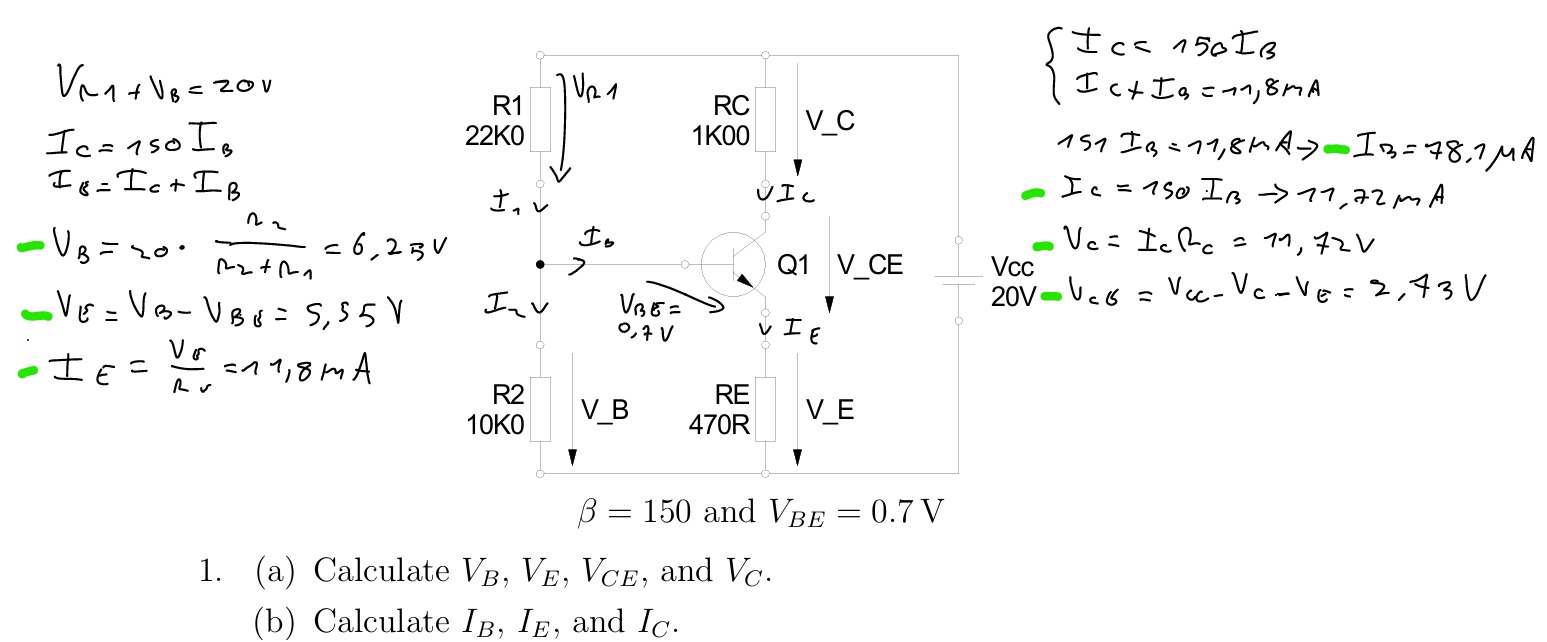
\includegraphics[scale=0.45]{prelab 3 ex 1 calc}\\
		\textbf{LTSpice simulation}\\\\
		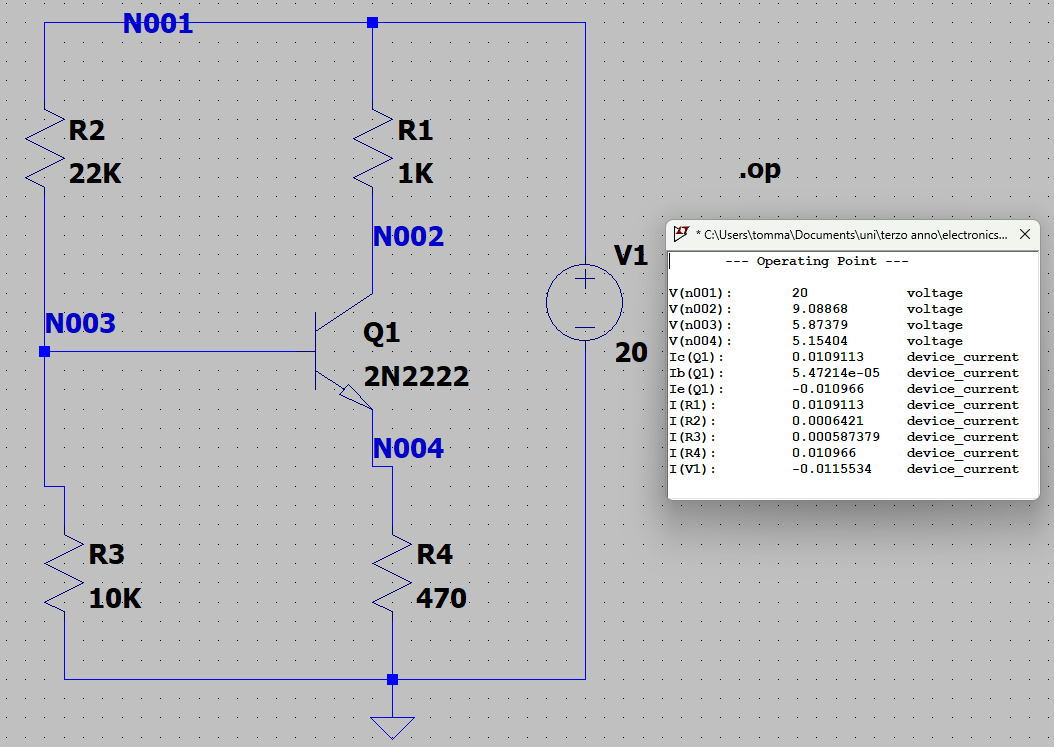
\includegraphics[scale=0.6]{prelab 3 ex1 circuit}\\
	\end{enumerate}
 	\pagebreak
	\subsection{Constant Current Source}
		\begin{enumerate}
			\item \textbf{Calculations and simulation on LTSpice}\\\\
			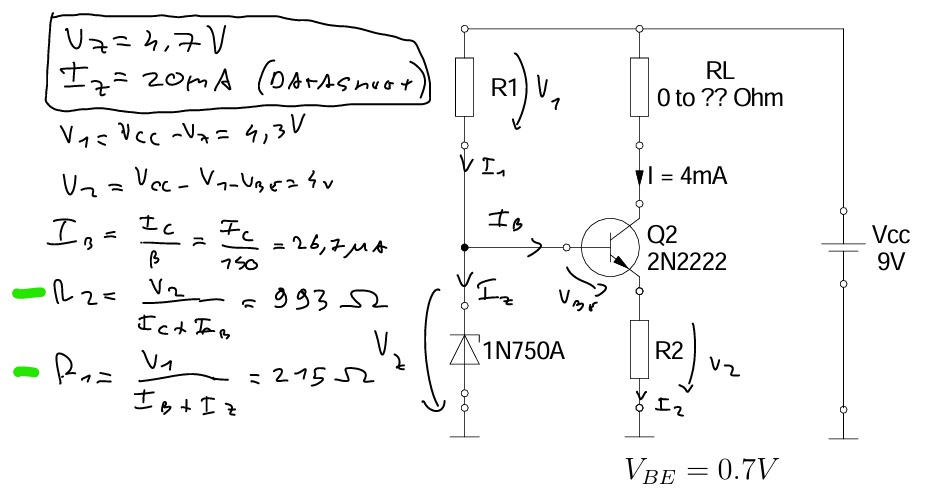
\includegraphics[scale=0.55]{prelab 3 ex2 calc}\\
			\item R1 = 215\(\Omega\), R2 = 993\(\Omega\)\\\\\\
			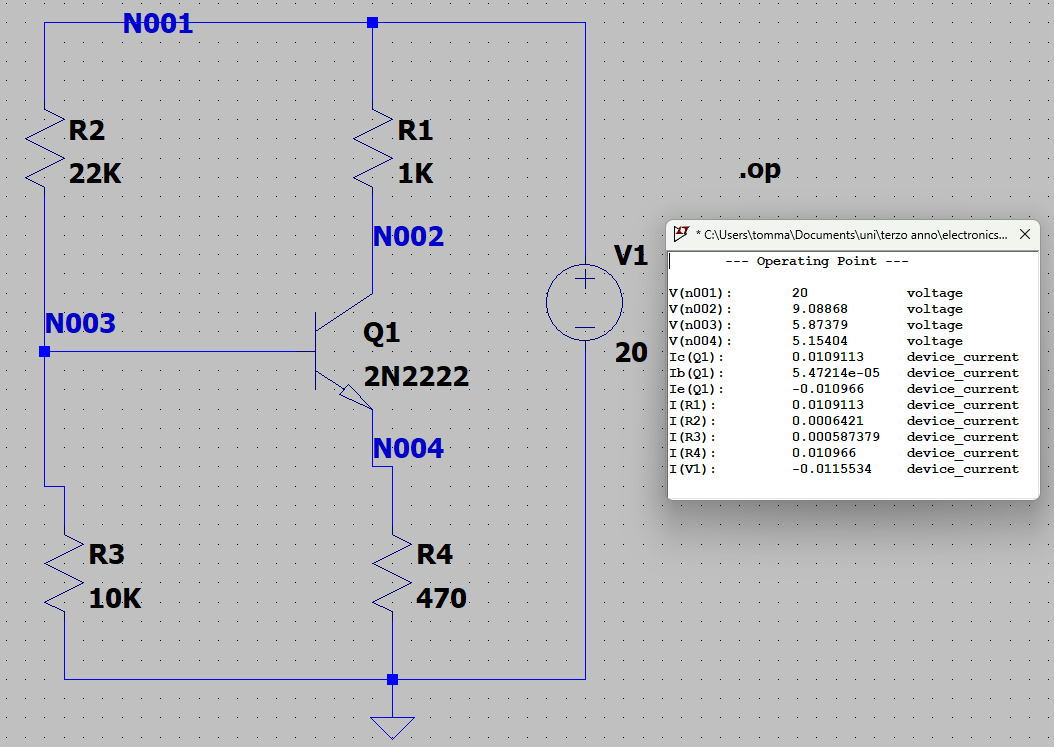
\includegraphics[scale=0.6]{prelab 3 ex1 circuit}\\\\
			\item To have a constant current \(V_{CE}\) has to be higher than 0.3V (from 2N2222 datasheet) to stay in active mode. So the condition for RL is \(V_{RL} < V_{CC}-0.3V-V_2 = V_{RL} < 4.7V\) so \(R_L\) must be lower than \(\frac{4.7}{0.004} \) = 1175 \(\Omega\).\\\\
			\pagebreak
			\item  \textbf{Max \(R_L\) in LTSpice}\\\\
			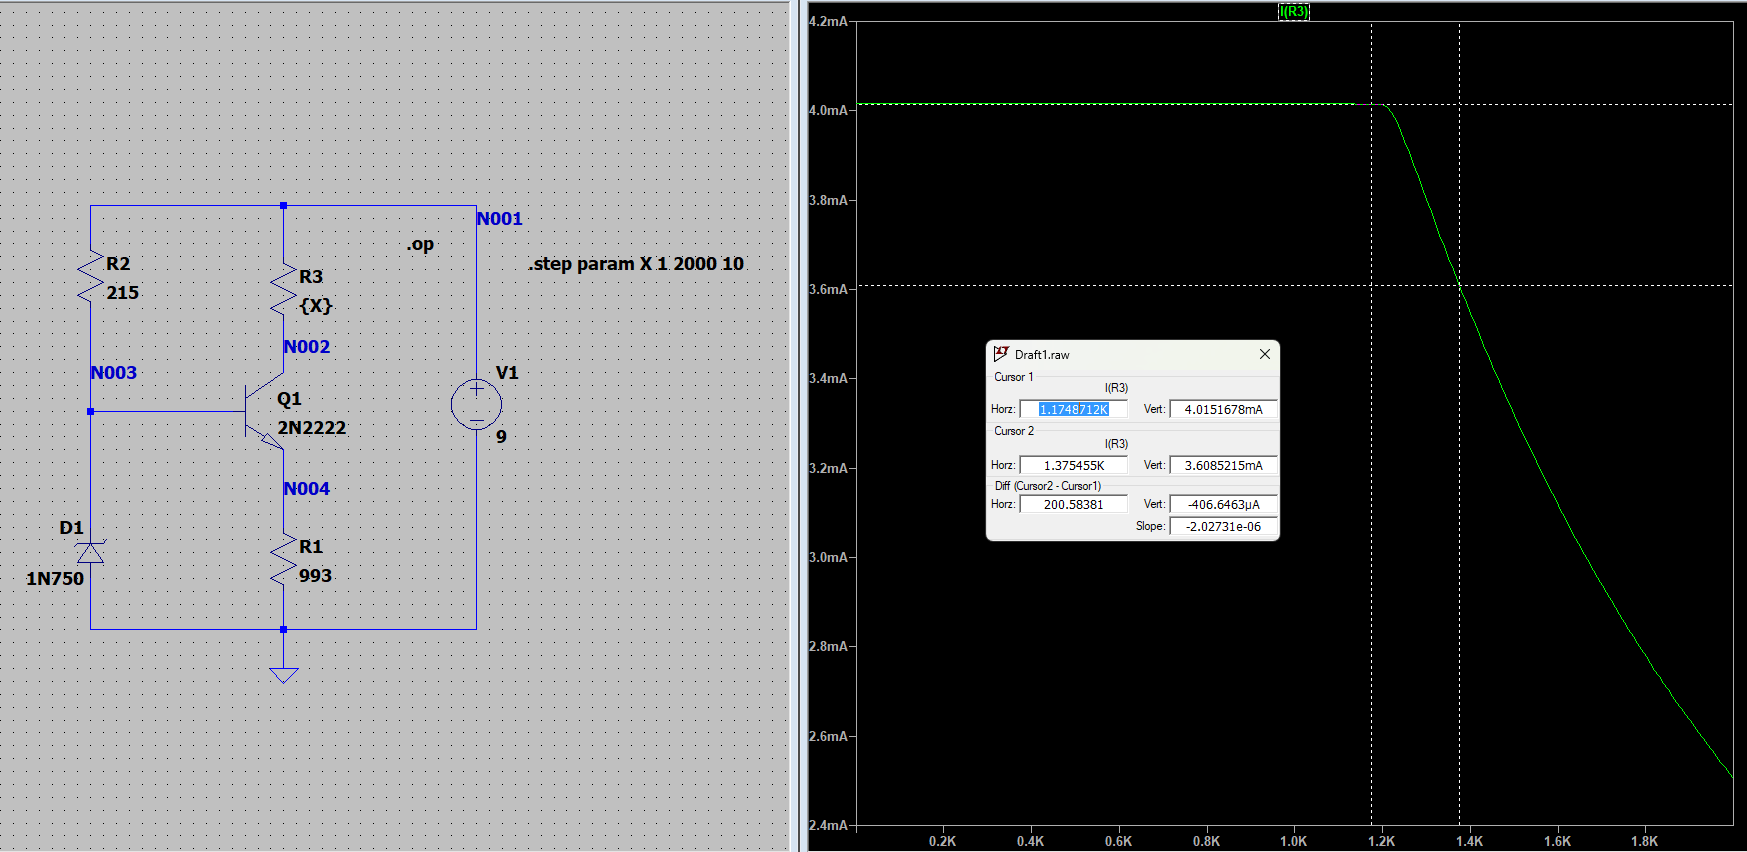
\includegraphics[scale=0.4]{prelab 3 ex2 rl}\\\\
			At 1275\(\Omega\) the current is 4mA, at 1375\(\Omega\) the current is 10\% less (3.6mA).  
		\end{enumerate}
	\subsection{Amplifier circuit}
		\begin{enumerate}
			\item 
			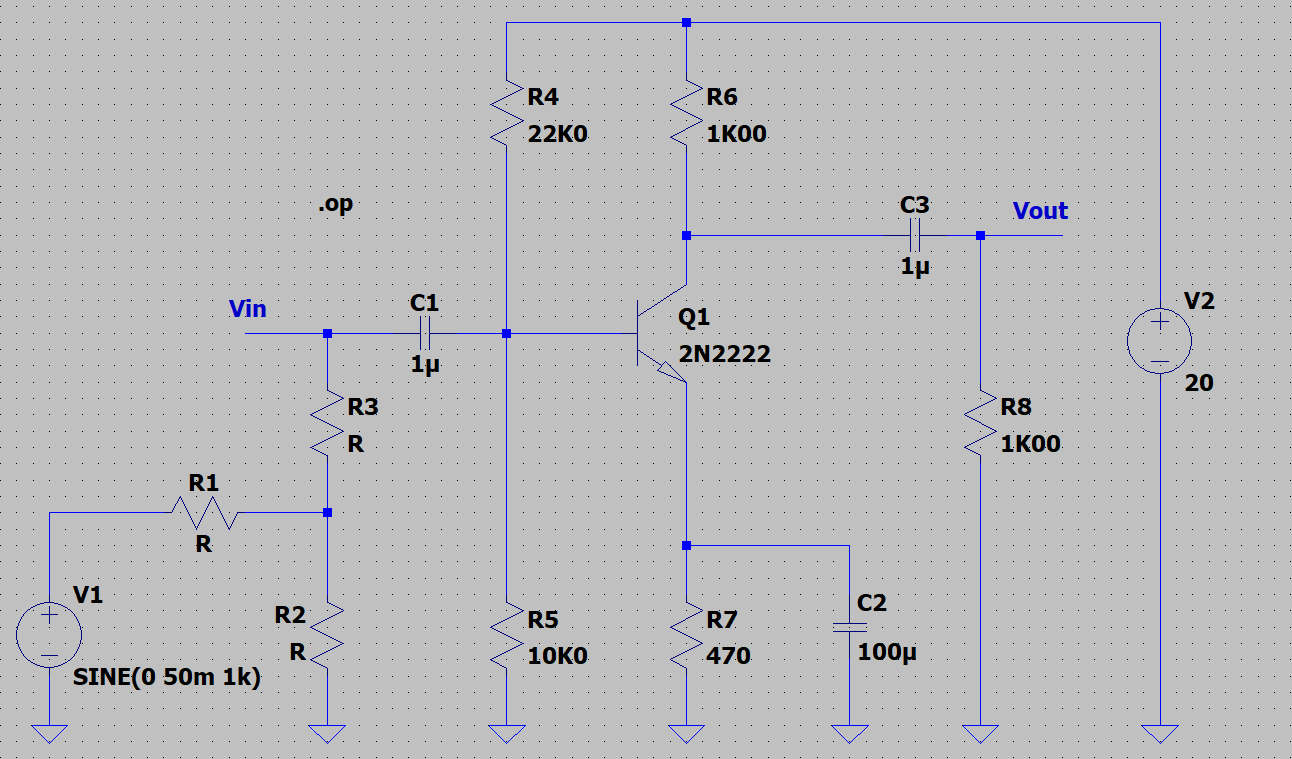
\includegraphics[scale=0.4]{prelab 3 ex3 circuit}\\\\
			\item \textbf{DC operation point values}\\\\
			\(I_C\) = 0.011 A, \(I_B\) = 54.7 uA\\
			\(V_B\) = 5.87V, \(V_E\) = 5.15 V, \(V_C\) = 9.09V, \(V_BE\) = 0.12, \(V_CE\) = 3.94V\\\\\pagebreak
			\item \textbf{Transient analysis at 50mV}\\\\
			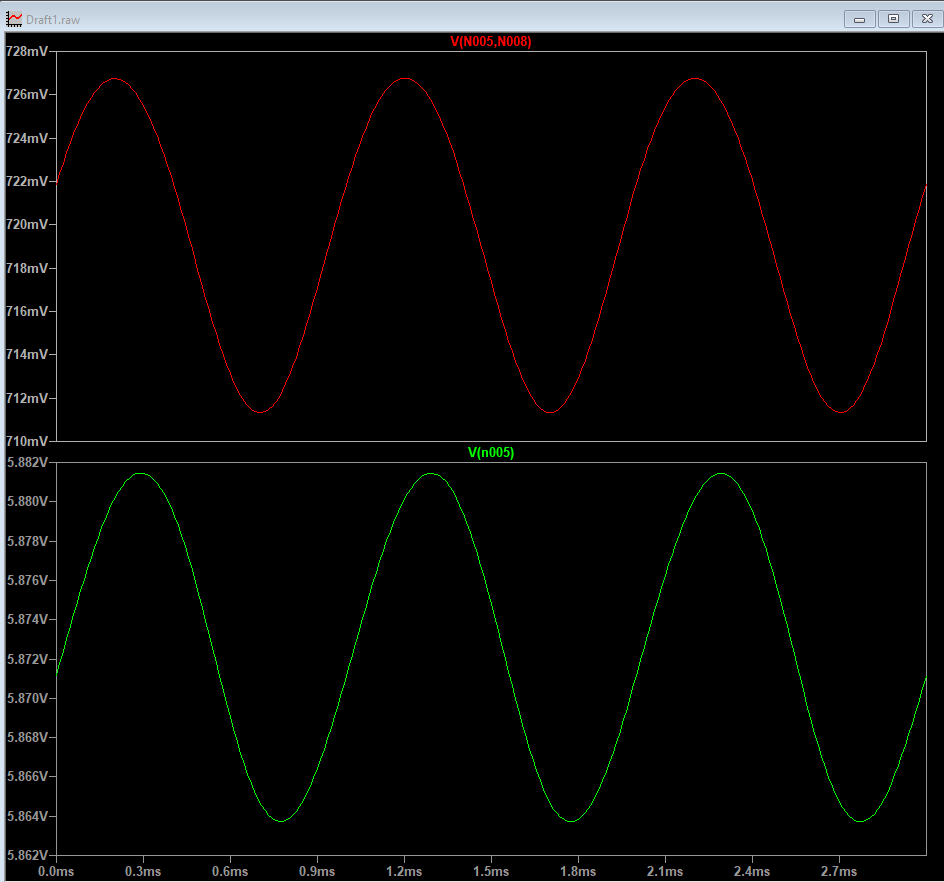
\includegraphics[scale=0.4]{prelab 3 ex3.3 1}\\\\
			Green line: \(V_B\): 17.7mV peak to peak, red line: \(V_{BE}\): 15.4mV peak to peak.\\\\
			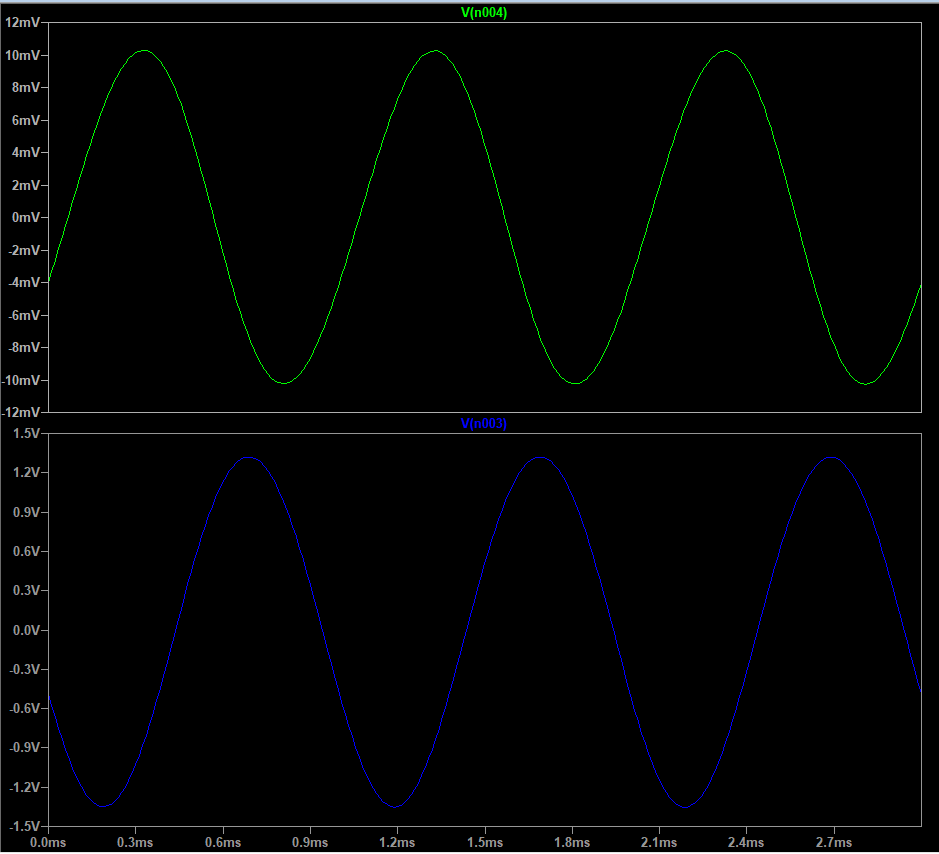
\includegraphics[scale=0.4]{prelab 3 ex3.3 2}\\\\
			Green line: \(V_i\): 20.5mV peak to peak, blue line: \(V_o\): 2.67V.\\\\ Gain: \(\frac{V_o}{V_i} = 130\).\pagebreak
			\item \textbf{Harmonic distortion analysis}\\\\
			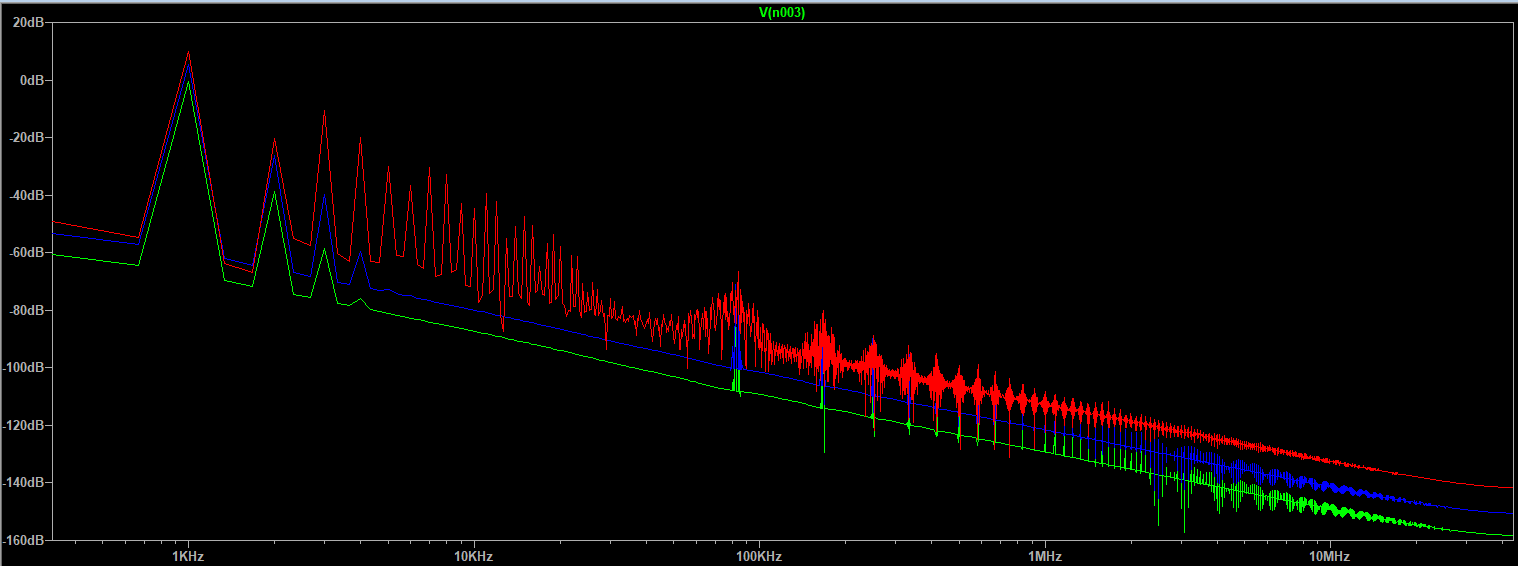
\includegraphics[scale=0.45]{prelab 3 ex3.4 1}\\\\
			According to the FFT the harmonic distortion is similar between 50mV and 100mV as input amplitude and is much worse when using 200mV.\\\pagebreak
			\item \textbf{AC analysis}\\\\
			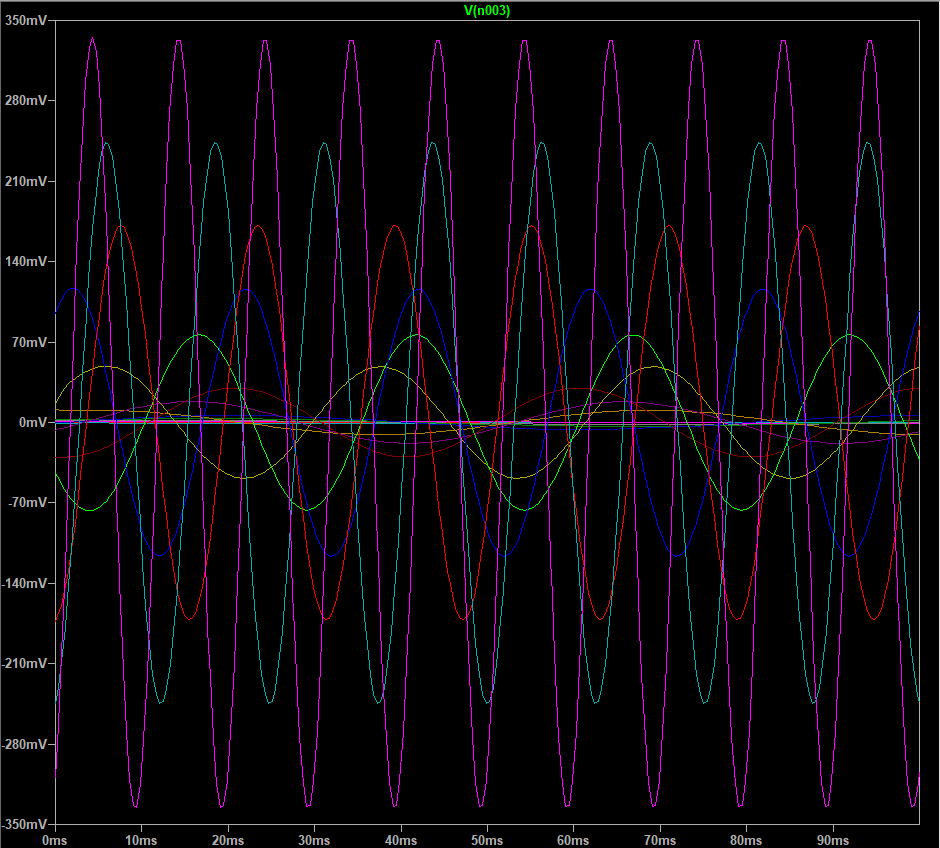
\includegraphics[scale=0.65]{prelab 3 ex3.5 1}\\\\
			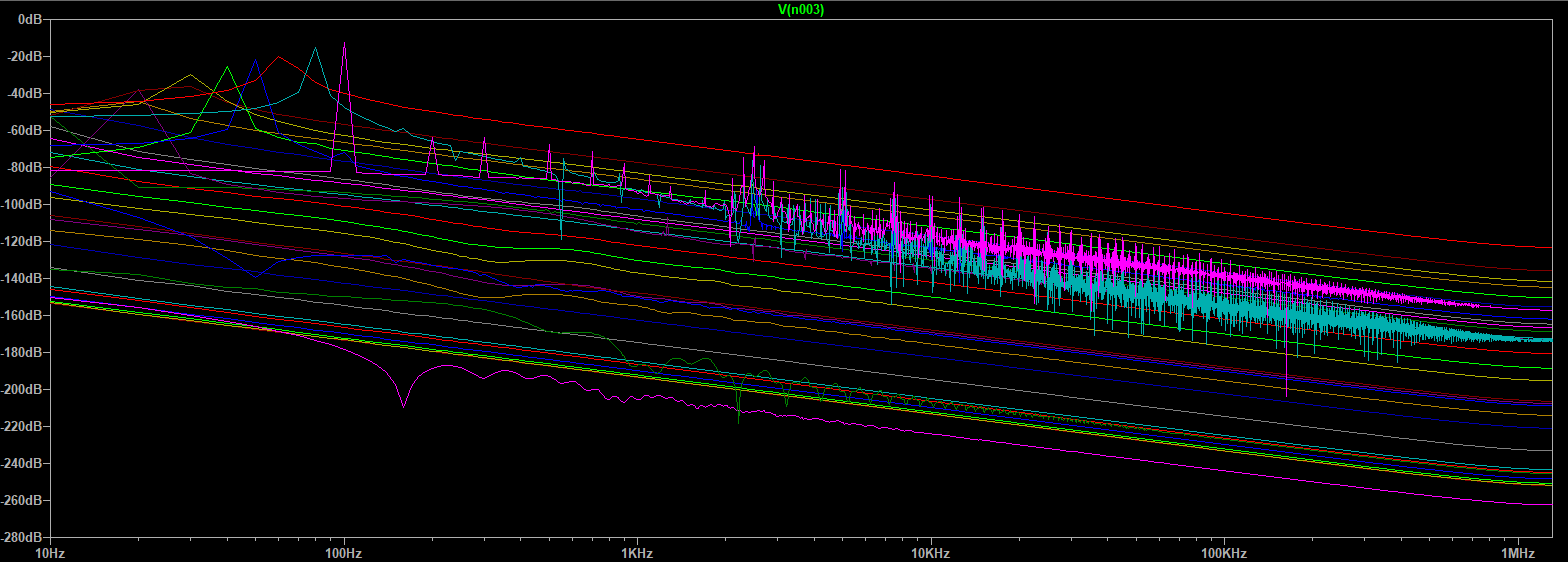
\includegraphics[scale=0.45]{prelab 3 ex3.5 2}\\\\\pagebreak
		\end{enumerate}
	
	
\end{document}